\chapter{Introduction}\label{chp:1}
Convolutional Neural Networks (CNNs) are a type of deep learning model \textbf{designed to recognize patterns in visual data}, such as images and videos. Unlike traditional neural networks, CNNs exploit the spatial and hierarchical patterns present in the data to efficiently learn features. CNNs consist of layers that perform convolutions, mathematical operations that filter and extract features such as edges, textures, and shapes from images. These networks typically have three main types of layers: \textbf{convolutional layers}, \textbf{pooling layers} (to reduce the image size), and \textbf{fully connected layers} (for final classification). CNNs are particularly powerful for tasks like image recognition, object detection, and facial recognition, as they automatically learn relevant features from the raw input data.

% Adding a figure
\begin{figure}[h!]
    \centering
    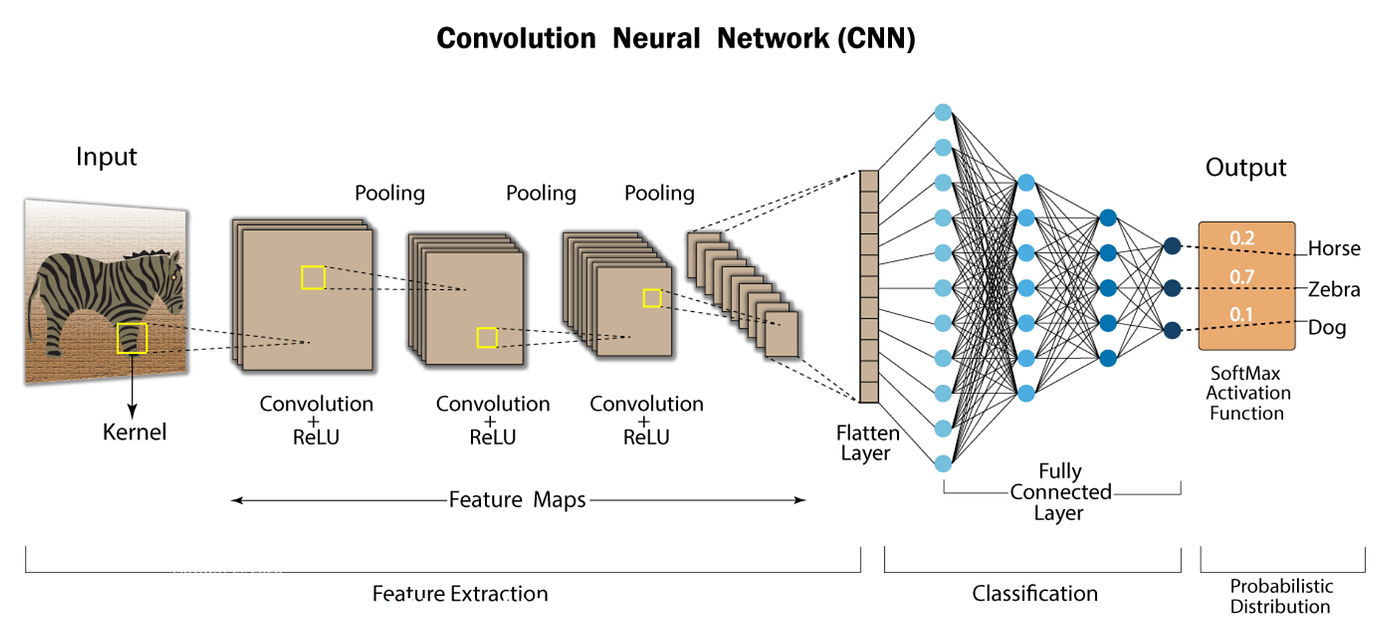
\includegraphics[width=0.9\textwidth]{images/figure1.png}
    \caption{A typical Convolutional Neural Network}
    \label{fig:1}
\end{figure}

\section{Key Characteristics of CNNs}
\begin{itemize}
    \item \textbf{Convolutions}: A mathematical operation that extracts patterns such as edges and textures.
    \item \textbf{Hierarchical Feature Learning}: CNNs learn low-level features (e.g., edges) in initial layers and complex patterns (e.g., objects) in deeper layers.
    \item \textbf{Parameter Sharing}: Convolutions reduce the number of parameters, making them computationally efficient.
    \item \textbf{Translation Invariance}: Recognize patterns regardless of their position in the input.
\end{itemize}
For instance, CNNs are capable of classifying an image of a cat even if the cat appears in different parts of the image.

\section{Why CNNs are important in Machine Learing}
A \textbf{Convolutional Neural Network (ConvNet/CNN)} can take in an input image, assign importance (learnable weights and biases) to various aspects/objects in the image, and be able to differentiate one from the other. \textbf{The pre-processing required in a ConvNet is much lower as compared to other classification algorithms}. While in primitive methods, filters are hand-engineered; with enough training, ConvNets have the ability to learn these filters/characteristics.\\

CNNs have revolutionized the field of computer vision and beyond by enabling machines to:
\begin{itemize}
    \item \textbf{Understand visual content}: Perform image classification, object detection, and segmentation.
    \item \textbf{Process structured data efficiently}: Learn features directly from raw input, reducing the need for manual feature engineering.
    \item \textbf{Achieve human-level accuracy}: Outperform traditional methods in tasks like face recognition, medical imaging, and natural language processing.
\end{itemize}

The architecture of a ConvNet is analogous to that of the connectivity pattern of Neurons in the Human Brain and was inspired by the organization of the Visual Cortex. Individual neurons respond to stimuli only in a restricted region of the visual field known as the Receptive Field. A collection of such fields overlaps to cover the entire visual area.

\section{Why ConvNets over Feed-Forward Neural Nets?}
An image is nothing but a matrix of pixel values. So why not just flatten the image (e.g. 3x3 image matrix into a 9x1 vector) and feed it to a Multi-Level Perceptron for classification purposes?\\

For extremely basic binary images, this method might show an average precision score while class prediction but would fail miserably for complex images with dependent pixels.

% \newpage
\begin{figure}[h!]
    \centering
    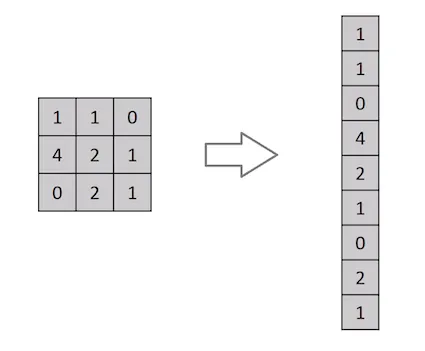
\includegraphics[width=0.35\textwidth]{images/figure2.png}
    \caption{Flattening of a 3x3 image matrix into a 9x1 vector}
    \label{fig:2}
\end{figure}

A ConvNet can \textbf{successfully capture the Spatial and Temporal dependencies} in an image through the application of relevant filters. The architecture performs a better fitting to the image dataset due to the reduction in the number of parameters involved and the reusability of weights.\\

\fbox{%
    \parbox{\textwidth}{%
        \textbf{Spatial Dependency} means a pixel's value is influenced by nearby pixel's value in image. This is because generally they all belong to same color because they are from same object. \textbf{Temporal dependency} comes in videos. When a frame changes to next, if there is not a lot of movement in objects, pixel's values remain same.
    }%
}
\begin{table}[h!]
\centering
\begin{tabular}{|p{0.25\linewidth}|p{0.32\linewidth}|p{0.32\linewidth}|} 
  \hline
  \rowcolor{lightgray} \textbf{Aspect} & \textbf{ANN} & \textbf{CNN} \\ 
  \hline\hline
  \textbf{Input Representation} & Flat, requires feature extraction & Structured (e.g., images as grids of pixels) \\ 
  \hline
  \textbf{Architecture} & Fully connected layers & Convolutional + pooling layers + fully connected layers \\ 
  \hline
  \textbf{Parameter Count} & High (independent weights for each connection) & Low (shared weights through convolutions) \\
  \hline
  \textbf{Feature Learning} & Manual or less efficient & Automatic and hierarchical \\
  \hline
  \textbf{Applications} & Generic machine learning & Specialized for spatial and structured data \\
  \hline
\end{tabular}
\caption{Difference between ANNs and CNNs}
\label{table:1}
\end{table}

\section{Visual Representation of CNN workflow}
The image illustrates a simple Convolutional Neural Network (CNN) designed to classify handwritten digits from the \textbf{MNIST dataset}. The MNIST dataset contains $28 \times 28$ grayscale images of handwritten digits, with the goal to classify them into one of the $10$ output classes (from $0$ to $9$), i.e., to predict which digit (from $0$ to $9$) is represented in each image. Below are the sequence of layers the input images are passed through:\\

\textbf{Input Layer}:
Each input image is $28 \times 28$ pixels, where each pixel represents a grayscale value ranging from $0$ (black) to $255$ (white). The input image is then fed into the CNN for processing.\\

\textbf{Convolutional Layer}:
The first step in the CNN is the convolutional layer, where a set of small filters or kernels is applied to the input image. These filters scan the image and detect basic features like edges or corners. This process results in feature maps that highlight the presence of certain features in different parts of the image.\\

\textbf{Pooling Layer}:
Next, a pooling layer reduces the spatial dimensions of the feature maps, typically using max pooling. This operation retains the most important information while reducing the amount of data, making the network more computationally efficient.\\

\textbf{Flattening and Fully Connected Layers}:
After pooling, the output is flattened into a one-dimensional vector and passed through fully connected layers. These layers combine the learned features and classify the image into one of the $10$ classes (digits $0$ to $9$).

% \newpage
\begin{figure}[h!]
    \centering
    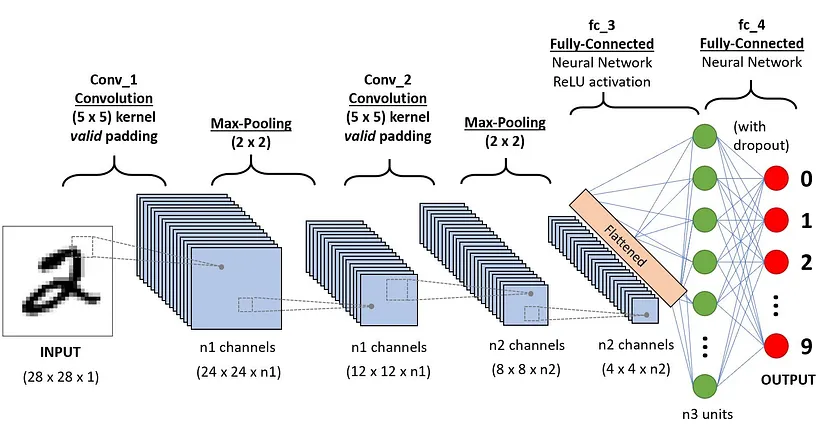
\includegraphics[width=0.9\textwidth]{images/figure3.png}
    \caption{A CNN architecture to classify handwritten digits from the MNIST dataset}
    \label{fig:3}
\end{figure}

\textbf{Output Layer}:
The final layer is the output layer, where a \textbf{softmax} activation function assigns probabilities to each class. The class with the highest probability is the predicted digit.\\

\textbf{Training and Classification}:
The CNN is trained using labeled MNIST images and adjusts its internal parameters through backpropagation to minimize prediction errors. Once trained, the model can accurately classify unseen handwritten digits.


